\documentclass[11pt,addpoints]{exam}
\usepackage{enumitem}
\usepackage{amsfonts,amssymb,amsmath, amsthm}
\usepackage{graphicx}
\usepackage{systeme}
\usepackage{pgf,tikz,pgfplots}
\pgfplotsset{compat=1.15}
\usepgfplotslibrary{fillbetween}
\usepackage{mathrsfs}
\usetikzlibrary{arrows}
\usetikzlibrary{calc}
\pagestyle{headandfoot}
%\firstpageheadrule
\runningheader{Homework 6}{}{Page \thepage\ of \numpages}
\runningheadrule
\author{Aaron GK}
\usepackage{geometry}
\geometry{
	a4paper,
	total={170mm,257mm},
	left=15mm,
	right=15mm,
	bottom=20mm,
	top=15mm,
}
\firstpagefooter{}{}{}
\runningfooter{}{}{}


\begin{document}
	\title{St John Baptist De La Salle Catholic School, Addis Ababa\\
		\large Homework 6 Solution\\
		3rd Quarter}
	\maketitle
	\begin{center}
		\fbox{\fbox{\parbox{6in}{\centering
					Notes, and use of other aids is allowed.  Read all directions carefully and write your answers in the space provided.  To receive full credit, you must show all of your work. \textbf{Cheating or indications of cheating and similar answers will be punished accordingly}. 
		}}}
		\subsubsection*{Information}
		\begin{itemize}
			\item The homework is due on \textbf{Wednesday}, \textbf{April 05}.
			\item You should Work on it \textbf{in groups} and consult me if you have any questions. Cheating within groups is unacceptable.
			\item For purposes of neatness and simplicity of grading, you should do the homework on an \textbf{A-4 paper}.
		\end{itemize}
	\end{center}
	\begin{center}
		\subsection*{Questions}
	\end{center}
	\begin{questions}
		\question An electrical generator is made of a circular coil of 0.50m radius. If there are 500 turns of the coil and it is rotating at a rate of 4000 rpm in a 1.800 T field, answer the following questions.
		\begin{enumerate}[label=(\alph*)]
			\item Write the emf as a function of time. \\ \textbf{Answer} \\ \\
			$$\mathcal{E}=NAB\omega\sin(\omega t)$$
			We should express the quantities in their standard units first. Thus
			$$\omega= 4000 rpm = 4000 \times \dfrac{2\pi}{60}rad/s=\dfrac{400\pi}{3}rad/s$$
			$$A=\pi r^2=\pi(0.5m)^2=0.25\pi m^2$$
			$$\mathcal{E}=500\times(0.25\pi m^2)\times1.800T\times\dfrac{400\pi}{3}rad/s\sin(\dfrac{400\pi}{3}t)$$
			\item What is the maximum emf?
			The maximum emf is reached when $\sin(\omega t)=1$, which gives us that $\mathcal{E}=NAB\omega$.
			$$\mathcal{E}=500\times(0.25\pi m^2)\times1.800T\times\dfrac{400\pi}{3}rad/s$$
		\end{enumerate}
		\question The Concorde had a wingspan of 26m and it could fly up to speeds of Mach 2. 
		\begin{enumerate}[label=(\alph*)]
			\item What emf is induced between wing tips if the vertical component of the Earth’s field is $3\times10^{-5}T$?
			\\ \textbf{Answer} \\ \\
			This is the case of a motional emf and the induced emf is given by
			$$\mathcal{E}=Blv$$
			$$\mathcal{E}=3\times10^{-5}T\times26m\times686m/s$$
			\textbf{Note:} Mach is a measurement of speed in relation to the speed of sound in air. Mach 1 is the speed of sound in air, while Mach 2 is twice the speed of sound in air and goes on. 
			\item Discuss if the induced emf would have a significant effect on the workings of the plane. \\ \textbf{Answer} \\
			The induced emf is very small to cause any significant to the plane or the travelers.
		\end{enumerate}
		\question A large power plant generates electricity at 25.0 kV. An old transformer once converted the voltage to 335 kV. The secondary of this transformer is being replaced so that its output can be 850 kV for more efficient transmission.
		\begin{enumerate}[label=(\roman*)]
			\item What is the ratio of turns in the new secondary compared with the old secondary? \\ \textbf{Answer} \\ \\
			$$\dfrac{Vs_{old}}{Ns_{old}}=\dfrac{Vp}{Np}$$
			$$Ns_{old}=\dfrac{Vs_{old}}{Vp}Np$$
			However when the transformer secondary coils are replaced, the primary coils and the input are the same. Thus, we have:
			$$\dfrac{Vs_{new}}{Ns_{new}}=\dfrac{Vp}{Np}$$
			$$Ns_{new}=\dfrac{Vs_{new}}{Vp}Np$$
			Now, we can find the ratio
			$$\dfrac{Ns_{new}}{Ns_{old}}=\dfrac{\dfrac{Vs_{new}}{Vp}Np}{\dfrac{Vs_{old}}{Vp}Np}=\dfrac{Vs_{new}}{Vs_{old}}$$
			$$\dfrac{Ns_{new}}{Ns_{old}}=\dfrac{Vs_{new}}{Vs_{old}}=\dfrac{850kV}{335kV}=\dfrac{850}{335}$$
			\item What is the ratio of new current output to old output for the same power? 
			$$\dfrac{Is_{new}}{Ip}=\dfrac{Np}{Ns_{new}}$$
			$$Is_{new}=\dfrac{Np}{Ns_{new}}Ip$$
			But, before the secondary coils were replaced, the output current was
			$$\dfrac{Is_{old}}{Ip}=\dfrac{Np}{Ns_{old}}$$
			$$Is_{old}=\dfrac{Np}{Ns_{old}}Ip$$
			Which gives us the ratio below
			$$\dfrac{Is_{new}}{Is_{old}}=\dfrac{\dfrac{Np}{Ns_{new}}Ip}{\dfrac{Np}{Ns_{old}}Ip}$$
			$$\dfrac{Is_{new}}{Is_{old}}=\dfrac{Ns_{old}}{Ns_{new}}=\dfrac{335}{850}$$
		\end{enumerate} 
		\question An RL circuit is made of an inductor of 20mH and a resistor of 20 $\Omega$ that are connected in series. If the circuit includes a battery of 20 V of emf, 
		\begin{enumerate}[label=(\roman*)]
			\item Write the current and emf as functions of time.
			$$\mathcal{E}(t)=\mathcal{E}(1-e^{-{\frac{tR}{L}}})$$
			$$\mathcal{E}(t)=20V(1-e^{-{\frac{t20\Omega}{20mH}}})$$
			$$\mathcal{E}(t)=20(1-e^{-1000t})V$$
			$$I(t)=\dfrac{\mathcal{E}(t)}{R}=\dfrac{20(1-e^{1000t})V}{20\Omega}$$
			$$I(t)=(1-e^{1000t})A$$
			\item Find the induced EMF 8.00 ms after the switch is turned on.
			$$\mathcal{E}(8ms)=20(1-e^{1000(0.008)})V$$
			$$\mathcal{E}(8ms)=20(1-e^{-8})V$$
			\item What direction is the current acting?	\\ \\
			Until the emf reaches its maximum value in the inductor, the current will be increasing in the circuit.
		\end{enumerate} 
		\subsection*{Advanced Problems}
		\question A square loop of side 10 cm is placed 2 cm from a long wire carrying a current that varies with time at a constant rate of 3 A/s as shown in the figure below.
		\begin{center}
			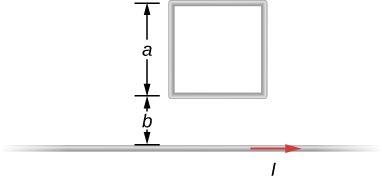
\includegraphics[scale=1]{1}
		\end{center} 
		\begin{enumerate}[label=(\roman*)]
			\item Use Ampère’s law and find the magnetic field. 
			\item Determine the magnetic flux through the loop.
			\item If the loop has a resistance of 3$\Omega$, how much induced current flows in the loop? 
		\end{enumerate}
	\end{questions}		
\end{document}